\documentclass{article}
\usepackage{titlesec}
\usepackage{xcolor}
\usepackage{microtype}
\usepackage{subfigure}
\usepackage{booktabs}
\usepackage{hyperref}
\usepackage{siunitx}
\usepackage{graphicx}
\usepackage{amsmath}
\usepackage[capitalize,noabbrev]{cleveref}
\usepackage{hyperref}
\usepackage{amssymb}
\usepackage{mathtools}
\usepackage{amsthm}
\usepackage{url}
\def\UrlBreaks{\do\/\do-}
\usepackage{tikz}
\usepackage{xfrac}
\usepackage{multirow}
\usepackage[inline]{enumitem}
\usepackage{todonotes}
\usepackage{pgfplots}
\usepackage{pgfplotstable}
\usepackage{caption}
\usepackage{subfigure}
\usepackage{bbm}
\usepackage{setspace}

\usepackage[utf8]{inputenc}  % For LaTeX (older versions)
\usepackage[T1]{fontenc}      % Recommended for special characters

%\usepackage{icml2024}
\usepackage[accepted]{icml2024} 


\pgfplotsset{compat=1.16}

\usetikzlibrary{patterns}
\usetikzlibrary{shapes, arrows.meta, positioning}
\DeclareSIUnit\token{tok}
\DeclareSIUnit\sample{sam}
\sisetup{
group-separator={\,},
group-minimum-digits=4
}
\DeclareMathOperator{\diag}{diag}
\DeclareMathOperator{\macs}{MACs}
\newcommand\norm[1]{\left\lVert#1\right\rVert}
\DeclareSIUnit{\spike}{spike}
\DeclareSIUnit{\messages}{messages}

\DeclareSIUnit{\million}{M}
\DeclareSIUnit{\billion}{B}
\definecolor{color1}{HTML}{E41A1C}
\definecolor{color2}{HTML}{377EB8}
\definecolor{color3}{HTML}{4DAF4A}
\definecolor{color4}{HTML}{984EA3}
\definecolor{color5}{HTML}{FF7F00}

\definecolor{lightblue}{RGB}{119,170,221}
\definecolor{lightcyan}{RGB}{153,221,255}
\definecolor{mint}{RGB}{68,187,153}
\definecolor{pear}{RGB}{187,204,51}
\definecolor{olive}{RGB}{170,170,0}
\definecolor{lightyellow}{RGB}{238,221,136}
\definecolor{orange}{RGB}{238,136,102}
\definecolor{pink}{RGB}{255,170,187}
\definecolor{palegrey}{RGB}{221,221,221}

\icmltitlerunning{Accelerating Linear RNNs at the Edge with Unstructured Sparsity}
% Scalability of linear recurrent neural networks with unstructured sparsity
% Scalable and efficient linear recurrent neural networks with unstructured sparsity
% Scalable linear recurrent neural networks with 10x sparsity


%•  "Modern Linear RNNs for Streaming Inference: Fast and Energy-Efficient Solutions for Edge Devices"
%•  "Signal Processing with Modern RNNs: Low-Latency Streaming Inference on Neuromorphic Processors"
%•  "Unstructured Sparsity in Linear RNNs: Enabling Energy-Efficient Streaming Inference at the Edge"
%•  "Low-Latency and Energy-Efficient Signal Processing with Modern RNNs for Edge Applications"
%•  "Neuromorphic-Friendly Linear RNNs for Streaming Inference with Unstructured Sparsity"
%•  "Fast and Efficient Linear RNNs for Streaming Signal Processing on Edge Devices"
%•  "Streaming Signal Processing with Energy-Efficient Linear RNNs on Neuromorphic Hardware"
%•  "Unstructured Sparsity in Modern RNNs: Optimizing Low-Latency Edge Inference"
%•  "Energy-Efficient Linear RNNs: Streaming Signal Processing for Neuromorphic Processors"
%•  "Modern RNNs for Real-Time Edge Inference: Signal Processing with Low Latency and High Efficiency"
%•  "Modern Linear RNNs for Streaming Inference on Edge Devices with Unstructured Sparsity"
%•  "Energy-Efficient Signal Processing with Neuromorphic Processors and Low-Latency Modern RNNs"
%•  "Hardware-Aware Design of Linear RNNs for Fast, Low-Latency Streaming Inference"
%•  "Unstructured Sparsity in Modern RNNs for Energy-Efficient Edge Computing"
%•  "Neuromorphic Signal Processing: Leveraging Modern RNNs for Fast, Energy-Efficient Streaming"
%•  "Edge-Optimized Linear RNNs: A Hardware-Aware Approach to Low-Latency Signal Processing"
%•  "Energy-Efficient Streaming Inference with Linear RNNs and Unstructured Sparsity"
%•  "Hardware-Aware Modern RNNs for Low-Latency, Fast Streaming Inference on the Edge"
%•  "Signal Processing Meets Edge AI: Efficient Neuromorphic Linear RNNs for Streaming Tasks"
%•  "Unleashing Energy Efficiency and Speed: Linear RNNs for Neuromorphic Processors"

\begin{document}

\twocolumn[
\icmltitle{Accelerating Linear Recurrent Neural Networks for the Edge\\ with Unstructured Sparsity}
%\icmltitle{Unstructured Sparsity Accelerates Linear Recurrent Neural Networks for the Edge on Neuromorphic Processors}

\icmlsetsymbol{equal}{*}
\begin{icmlauthorlist}
\icmlauthor{Alessandro Pierro}{equal,intel,lmu}
\icmlauthor{Steven Abreu}{equal,intel,groningen}
\icmlauthor{Jonathan Timcheck}{intel}
\icmlauthor{Philipp Stratmann}{intel}
\icmlauthor{Andreas Wild}{intel}
\icmlauthor{Sumit Bam Shrestha}{intel}
\end{icmlauthorlist}

\icmlaffiliation{intel}{Neuromorphic Computing Lab, Intel Corporation, USA}
\icmlaffiliation{lmu}{Institute of Informatics, LMU Munich, Germany}
\icmlaffiliation{groningen}{Bernoulli Institute \& CogniGron, University of Groningen, Netherlands}

\icmlcorrespondingauthor{Alessandro Pierro}{alessandro.pierro@intel.com}

\icmlkeywords{recurrent neural network, sparsity, pruning, quantization, state space model, real-time processing, audio processing, model compression, hardware co-design}

\vskip 0.3in

\begin{abstract}
\begin{abstract}

Hierarchical clustering is a powerful tool for exploratory data analysis, organizing data into a tree of clusterings from which a partition can be chosen. This paper generalizes these ideas by proving that, for any reasonable hierarchy, one can optimally solve any center-based clustering objective over it (such as $k$-means). Moreover, these solutions can be found exceedingly quickly and are \emph{themselves} necessarily hierarchical. 
%Thus, given a cluster tree, we show that one can quickly generate a myriad of \emph{new} hierarchies from it. 
Thus, given a cluster tree, we show that one can quickly access a plethora of new, equally meaningful hierarchies.
Just as in standard hierarchical clustering, one can then choose any desired partition from these new hierarchies. We conclude by verifying the utility of our proposed techniques across datasets, hierarchies, and partitioning schemes.


\end{abstract}

\end{abstract}
]

\printAffiliationsAndNotice{\icmlEqualContribution} 


\section{Introduction}
\label{sec:introduction}
\section{Introduction}

% Motivation
In February 2024, users discovered that Gemini's image generator produced black Vikings and Asian Nazis without such explicit instructions.
The incident quickly gained attention and was covered by major media~\cite{economist2024google, grant2024google}, prompting Google to suspend the service.
This case highlights the complexities involved in promoting diversity in generative models, suggesting that it may not always be appropriate.
Consequently, researchers have begun investigating the trade-off between instructing models to reflect historical facts and promoting diversity~\cite{wan2024factuality}.
Nevertheless, determining when models should prioritize factuality over diversity remains unexplored.

\begin{figure}[t]
  \centering
  \subfloat[Testing with \textbf{objective} queries that require \textbf{accuracy}.]{
    \includegraphics[width=1.0\linewidth]{Figures/obj-cover.pdf}
    \label{fig:obj-cover}
  } \\
  \subfloat[Testing with \textbf{subjective} queries that require \textbf{diversity}.]{
    \includegraphics[width=1.0\linewidth]{Figures/subj-cover.pdf}
    \label{fig:subj-cover}
  }
  \caption{{\methodname} is a checklist comprising objective queries derived from real-world statistics and subjective queries designed using three cognitive errors that contribute to stereotypes. It includes queries designed for LLMs and T2I models.}
\end{figure}

% Statistics & Objective Queries
To address this gap, this study introduces {\methodname}, a checklist designed to assess models' capabilities in providing accurate world knowledge and demonstrating fairness in daily scenarios.
For world knowledge assessment, we collect 19 key statistics on U.S. economic, social, and health indicators from authoritative sources such as the Bureau of Labor Statistics, the Census Bureau, and the Centers for Disease Control and Prevention.
Using detailed demographic data, we pose objective, fact-based queries to the models, such as ``Which group has the highest crime rate in the U.S.?''—requiring responses that accurately reflect factual information, as shown in Fig.~\ref{fig:obj-cover}.
Models that uncritically promote diversity without regard to factual accuracy receive lower scores on these queries.

% Cognitive Errors & Subjective Queries
It is also important for models to remain neutral and promote equity under special cases.
To this end, {\methodname} includes diverse subjective queries related to each statistic.
Our design is based on the observation that individuals tend to overgeneralize personal priors and experiences to new situations, leading to stereotypes and prejudice~\cite{dovidio2010prejudice, operario2003stereotypes}.
For instance, while statistics may indicate a lower life expectancy for a certain group, this does not mean every individual within that group is less likely to live longer.
Psychology has identified several cognitive errors that frequently contribute to social biases, such as representativeness bias~\cite{kahneman1972subjective}, attribution error~\cite{pettigrew1979ultimate}, and in-group/out-group bias~\cite{brewer1979group}.
Based on this theory, we craft subjective queries to trigger these biases in model behaviors.
Fig.~\ref{fig:subj-cover} shows two examples on AI models.

% Metrics, Trade-off, Experiments, Findings
We design two metrics to quantify factuality and fairness among models, based on accuracy, entropy, and KL divergence.
Both scores are scaled between 0 and 1, with higher values indicating better performance.
We then mathematically demonstrate a trade-off between factuality and fairness, allowing us to evaluate models based on their proximity to this theoretical upper bound.
Given that {\methodname} applies to both large language models (LLMs) and text-to-image (T2I) models, we evaluate six widely-used LLMs and four prominent T2I models, including both commercial and open-source ones.
Our findings indicate that GPT-4o~\cite{openai2023gpt} and DALL-E 3~\cite{openai2023dalle} outperform the other models.
Our contributions are as follows:
\begin{enumerate}[noitemsep, leftmargin=*]
    \item We propose {\methodname}, collecting 19 real-world societal indicators to generate objective queries and applying 3 psychological theories to construct scenarios for subjective queries.
    \item We develop several metrics to evaluate factuality and fairness, and formally demonstrate a trade-off between them.
    \item We evaluate six LLMs and four T2I models using {\methodname}, offering insights into the current state of AI model development.
\end{enumerate}



\section{Compressing linear RNNs}
\label{sec:background}\label{sec:methodology}
\section{The Sequential Bottleneck in Large Model Inference}
\label{sec:sequential_bottleneck}

\subsection{Understanding Sequential Dependencies}
\label{sec:sequential_dependencies}

Modern LLMs, such as the Llama series~\cite{touvron2023llama,touvron2023llama2,dubey2024llama} and the GPT series~\cite{radford2019language,brown2020language}, are built on transformer architectures consisting of stacked decoder blocks. As shown in Figure~\ref{fig:architech}(a), each decoder block contains two fundamental components: a Self-Attention (SA) block and a feed-forward network (FFN). During execution, the input of the SA block is first multiplied with three weight matrices $W_{Q}$, $W_{K}$, and $W_{V}$, yielding the outputs termed query ($q$), key ($k$), and value ($v$), respectively.

\begin{figure*}
    \centering
    \includegraphics[width=0.9\linewidth]{figures/overview_llm_intro.pdf}
    \caption{(a) The Llama architecture consists of stacked transformer decoder blocks. (b) Each decoder block contains a self-attention (SA) block and feedforward (FFN) block. (c) During the decoding stage, tokens are generated auto-regressively.}
    \label{fig:architech}
\end{figure*}

The computation flow, detailed in Figure~\ref{fig:architech}(b), shows how query and key vectors compute attention scores through matrix multiplication. After softmax normalization, these scores weight the value vectors, producing the SA output through a weighted sum and residual connection. This SA output feeds into the FFN, typically implemented as either a standard MLP~\cite{radford2018improving, radford2019language} or gated MLP~\cite{liu2021pay, touvron2023llama,touvron2023llama2}, with multiple fully connected layers and activation functions like GeLU~\cite{hendrycks2016gaussian} or SiLU~\cite{elfwing2018sigmoid}.

The core challenge emerges during inference, which consists of two main phases: prefill and decoding. While the prefill phase can process input sequences in parallel, the decoding phase introduces a critical bottleneck. As shown in Figure~\ref{fig:architech}(c), the model must predict each token sequentially, using both current and previous token information through their Key and Value (KV) vectors. These KV vectors are cached for subsequent predictions, leading to significant memory access latency as the sequence length grows.

\subsection{Breaking Sequential Dependencies}
\label{sec:breaking_dependencies}

Traditional approaches to accelerating LM inference have focused on reducing computational costs through model compression, knowledge distillation, and architectural optimizations. However, these methods primarily address individual computation costs rather than the fundamental sequential dependency that requires each token to wait for all previous tokens.

\begin{figure}
    \centering
    \includegraphics[width=0.85\linewidth]{figures/sd_intro_new.pdf}
    \caption{Illustration of speculative decoding workflow.}
    \label{fig:sd_intro}
\end{figure}

Speculative decoding (SD)~\cite{stern2018blockwise} has emerged as a promising solution that directly targets this sequential bottleneck. As illustrated in Figure~\ref{fig:sd_intro}, this approach introduces a two-phase process where a smaller, faster \textit{draft model} first predicts multiple tokens in parallel, followed by verification using the target model. The draft model enables parallel token generation, breaking away from traditional token-by-token generation, while the target model's verification step maintains output quality through accept/reject decisions.

This strategy has proven particularly valuable for real-time applications like interactive dialogue systems, where response latency directly impacts user experience. The verification mechanism provides a crucial balance between generation speed and output quality, accepting correct predictions to maintain throughput while falling back to sequential generation when necessary to preserve accuracy.

While SD represents one successful approach to breaking sequential dependencies in autoregressive (AR) models, it belongs to a broader family of \textit{generation-refinement} methods. The following sections present a systematic taxonomy of these approaches, examining how different techniques balance the trade-offs between generation parallelism and output quality.



% \section{Methodology}
\begin{figure*}[ht]
    \centering
    \includegraphics[width=\textwidth, trim=79 280 93 123, clip]{figures/framework_img.pdf}
    \caption{The pipeline of the \ENDow{} framework 
    %where each component is specified in a given configuration. 
    which yields a downstream task score and a WER score of the transcript set input to the task. The pipeline is executed for several severeties of noising and types of cleaning techniques. %Acoustic noising is applied at $k$ intensities, providing $k+1$ audio versions (including the non-noised version), eventually producing $k+2$ transcript versions (including the source transcript). Applying transcript cleaning reveals the effect of \textit{types} of noise. 
    Resulting scores are plotted on a graph for the analyses, as in, e.g., \autoref{fig_cleaning_graphs}.}
    %The pipeline is executed on $k+1$ intensities of acoustic noising (including the non-noised version), producing $k+2$ scores for the downstream task (including execution on the source transcripts). This process eventually describes the effect of the \textit{intensity} of transcript noise on the downstream task. The process is repeated for $m$ cleaning techniques ($m+1$ when including no cleaning), to analyze the benefit of a cleaning approach and the effect of the \textit{types} of transcript noise.}
    \label{fig_framework}
\end{figure*}

\section{Methodology}
This section presents our neural approach to preconditioning PDEs. We begin by formulating the problem and discretizing the governing PDEs in Section~\ref{subsec:problem_formulation}, followed by an overview of the Neural Preconditioning Operator (NPO) framework in Section~\ref{subsec:npo_framework}. Next, we define the learning objectives for training the NPO in Section~\ref{subsec:learning_npo}, and conclude with a detailed description of the Neural Algebraic Multigrid (NAMG) Operator in Section~\ref{subsec:npo_amg}, which combines classical multigrid principles with neural attention for efficient coarse-grid correction.

\subsection{Problem Formulation}
\label{subsec:problem_formulation}
We consider PDEs on a domain \(D \subset \mathbb{R}^d\), with functions from the input and solution spaces \(\mathcal{A}(D; \mathbb{R}^{d_a})\) and \(\mathcal{U}(D; \mathbb{R}^{d_u})\), respectively. The operator \(\mathcal{G}: \mathcal{A} \to \mathcal{U}\) is expressed as an integral:
\begin{equation}
    \mathcal{G}a(\mathbf{x}) = \int_{D} \kappa(\mathbf{x}, \mathbf{y}) \, a(\mathbf{y}) \, d\mathbf{y},
\end{equation}
where \(\kappa: D \times D \to \mathbb{R}\) is the kernel function.

After discretization, the PDE leads to a sparse, symmetric positive definite (SPD) matrix \(A \in \mathbb{R}^{n \times n}\) and a right-hand side vector \(\mathbf{f} \in \mathbb{R}^n\). Our goal is to learn a preconditioner \(M = \mathcal{M}_{\theta}(A, \mathbf{f})\), defined by:
\begin{equation}
    M \;=\; \mathcal{M}_{\theta}(A),
\end{equation}

where \(\theta\) are the learned parameters. The preconditioner \(M\) is trained to remain SPD and efficient to apply, improving the condition number of \(A\) and accelerating iterative solvers.

\subsection{Neural Preconditioning Operator Framework}
\label{subsec:npo_framework}
Figure~\ref{fig:framework} illustrates the two-phase workflow of our Neural Preconditioning Operator (NPO) framework, consisting of \emph{training} (Figure~\ref{fig:framework}(a)) and \emph{solving} (Figure~\ref{fig:framework}(b)). 

During the training phase, the NPO takes the system matrix \(A\) and right-hand side vector \(f\) as inputs and generates an intermediate output, including a preconditioner matrix \(M\), the solution approximation \(u\), and residual \(r\). Three loss functions are used to guide the optimization: the \emph{data loss} (from \(u\) and \(f\)), \emph{residual loss} (from \(r\)), and \emph{condition loss} (from \(M\)). The NPO's parameters \(\theta\) are updated by minimizing the sum of these losses.

Once trained, the NPO is applied in the solving phase to accelerate iterative Krylov subspace methods (e.g., CG or GMRES). Given a new system \(A\mathbf{x} = \mathbf{b}\), the solver repeatedly uses the learned \(M\) to compute preconditioned residuals \(z = M r\), significantly reducing iteration counts and improving convergence efficiency across various PDE systems and mesh types.

\subsection{Learning Neural Preconditioner Operator}
\label{subsec:learning_npo}
To train a neural preconditioner \( \mathcal{M}_{\theta}(A) \), we define two complementary loss functions: a \emph{condition loss} and a \emph{residual loss}. These losses guide the preconditioner to behave like \( A^{-1} \), improving both the spectral properties of the system and solution accuracy.

\subsubsection{Condition Loss}

A preconditioner that approximates \( A^{-1} \) should ensure that \( A \mathcal{M}_{\theta}(A) \approx I \). A natural objective is to minimize:
\begin{equation}
    \label{eq:inverse_loss}
    \bigl\| I - A\,\mathcal{M}_{\theta}(A) \bigr\|_F^2.
\end{equation}
However, directly optimizing this matrix norm is computationally infeasible for large systems. Instead, we define a condition loss over sampled residuals \(\mathbf{r}_i\) to achieve a similar effect:
\begin{equation}
    \label{eq:condition_loss}
    \min_{\theta} \frac{1}{N} \sum_{i=1}^{N} \bigl\| \bigl(I - A_i\,\mathcal{M}_{\theta}(A_i)\bigr)\,\mathbf{r}_i \bigr\|_2^2.
\end{equation}

This condition loss indirectly improves the system's spectral properties, reducing the condition number of the preconditioned matrix and thereby accelerating convergence in iterative solvers.

\subsubsection{Residual Loss}

While the condition loss ensures better spectral properties, it does not directly assess how well the preconditioner solves the system for the right-hand side \(\mathbf{b}_i\). To address this, we define a residual loss that measures the accuracy of the preconditioner when applied to \(\mathbf{b}_i\):
\begin{equation}
    \label{eq:residual_loss}
    \min_{\theta \in \Theta} 
    \frac{1}{N}
    \sum_{i=1}^{N}
    \bigl\|
       A_{i}\mathcal{M}_{\theta}(A_i)\bigl(\mathbf{b}_i\bigr)
       \;-\;
       \mathbf{b}_i
    \bigr\|_2^2.
\end{equation}

This loss encourages \( \mathcal{M}_{\theta}(A) \) to approximate \( A^{-1} \) by minimizing the discrepancy between the predicted and actual right-hand side. Together, the condition and residual losses promote a preconditioner that reduces both spectral issues and iteration counts, enabling faster and more robust convergence for a wide range of PDE systems.

\subsection{Neural Algebraic Multigrid Operator}
\label{subsec:npo_amg}

The Neural Algebraic Multigrid (NAMG) Operator enhances the classical AMG framework by introducing neural attention mechanisms for efficient feature aggregation and prolongation. The process involves three main steps: restriction, attention-based coarse-grid correction, and prolongation.

\subsubsection{Restriction and Coarse Feature Aggregation}

Given fine-grid features \( \mathbf{x}^{f} \in \mathbb{R}^{N \times C} \) and the adjacency matrix \( A \in \mathbb{R}^{N \times N} \), restriction is defined as:

\begin{equation}
    \mathbf{x}^{c} = R \mathbf{x}^{f}, \quad R = A \cdot E_{\theta},
\end{equation}

where \( E_{\theta} \) contains learned attention weights:

\begin{equation}
    e_{ji} = \frac{\exp(\mathbf{W}_{\text{coarse}} \mathbf{x}_{i}^{f} / \tau)}{\sum_{i' \in \mathcal{N}_j} A_{ji'} \exp(\mathbf{W}_{\text{coarse}} \mathbf{x}_{i'}^{f} / \tau)}.
\end{equation}

Here, \( \mathcal{N}_j \) denotes the neighbors of node \( j \), \( \mathbf{W}_{\text{coarse}} \) is a learnable weight matrix, and \( \tau \) is a scaling parameter. Coarse features are computed by aggregating fine-grid tokens using these weights.

\subsubsection{Attention-Based Coarse Correction}

The coarse-grid features are refined through self-attention. Queries, keys, and values are computed as:

\begin{equation}
    \mathbf{q} = \mathbf{W}_{q} \mathbf{x}^{c}, \quad \mathbf{k} = \mathbf{W}_{k} \mathbf{x}^{c}, \quad \mathbf{v} = \mathbf{W}_{v} \mathbf{x}^{c}.
\end{equation}

Attention scores are then used to update the coarse features:

\begin{equation}
    \mathbf{x}_{j}^{c, \text{updated}} = \sum_{k} \text{softmax}\left( \frac{\mathbf{q}_{j} \cdot \mathbf{k}_{k}^{\top}}{\sqrt{C}} \right) \mathbf{v}_{k}.
\end{equation}

\subsubsection{Prolongation and Fine-Grid Correction}

The updated coarse features are projected back to the fine grid:

\begin{equation}
    \mathbf{x}'^{f} = \mathbf{x}^{f} + P \mathbf{x}'^{c}, \quad P = A \cdot E_{\theta}^{\top}.
\end{equation}

This process dynamically adjusts restriction and prolongation through learned attention, allowing the operator to capture complex patterns inherent in PDEs across diverse domains. 


\begin{figure*}[t]
    \centering
    \small
    \hspace*{-1.2cm}
    \subfigure[Alignment stage]{
    \begin{minipage}[t]{0.24\linewidth}
    \centering
      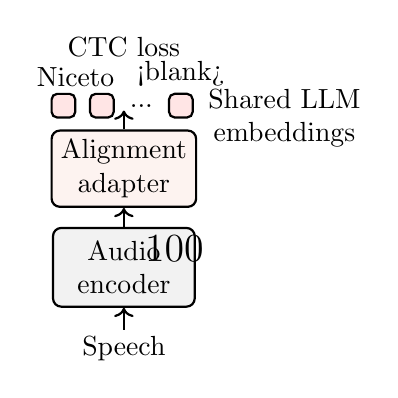
\begin{tikzpicture} [scale=0.8]
        \node(ae) at (0,0) [rectangle, draw=black, fill=gray!10, rounded corners=3pt, thick, minimum width=1.8cm,minimum height=1cm,align=center] {Audio\\encoder};
        \node(freeze) at ([xshift=0.8cm,yshift=0.3cm]ae.center) [rectangle, align=center] {\Large{\ding{100}}};
        \node(fb) at ([yshift=-0.3cm]ae.south) [rectangle, align=center,anchor=north] {Speech};
        \node(aa) at ([yshift=0.3cm]ae.north) [rectangle, draw=black, fill=orange!10, rounded corners=3pt, thick, minimum width=1.8cm,minimum height=0.5cm,align=center,anchor=south] {Alignment\\adapter};
        
        \node(f1) at ([yshift=1.0cm]aa.west) [rectangle, draw=black, fill=red!10, rounded corners=2pt, thick, minimum width=0.3cm, minimum height=0.3cm,align=center,anchor=west] {};
        \node(f2) at ([xshift=0.2cm]f1.east) [rectangle, draw=black, fill=red!10, rounded corners=2pt, thick, minimum width=0.3cm, minimum height=0.3cm,align=center,anchor=west] {};
        \node(f3) at ([xshift=0.075cm]f2.east) [rectangle, draw=white,  thick, align=center,anchor=west] {...};
        \node(f4) at ([xshift=0.075cm]f3.east) [rectangle, draw=black, fill=red!10, rounded corners=2pt, thick, minimum width=0.3cm, minimum height=0.3cm,align=center,anchor=west] {};
        \node(t1) at ([yshift=-0.05cm]f1.north) [rectangle, align=center,anchor=south] {Nice};
        \node(t2) at ([yshift=-0.05cm]f2.north) [rectangle, align=center,anchor=south] {to};
        \node(t4) at ([yshift=-0.05cm]f4.north) [rectangle, align=center,anchor=south] {<blank>};
        \node(se) at ([xshift=0.075cm,yshift=-0.2cm]f4.east) [rectangle, align=center,anchor=west] {Shared LLM\\embeddings};
        \node(ctc) at ([yshift=1.0cm]aa.north) [rectangle, rounded corners=3pt, thick, align=center,anchor=south] {CTC loss};

        
        \draw[->,thick]([yshift=-0.05cm]fb.north)--(ae.south);
        \draw[->,thick](ae.north)--(aa.south);
        \draw[->,thick](aa.north)--([yshift=0.3cm]aa.north);

        
      \end{tikzpicture}
    \end{minipage}
    }
    \subfigure[Shrinking stage]{
    \begin{minipage}[t]{0.45\linewidth}
    \centering
    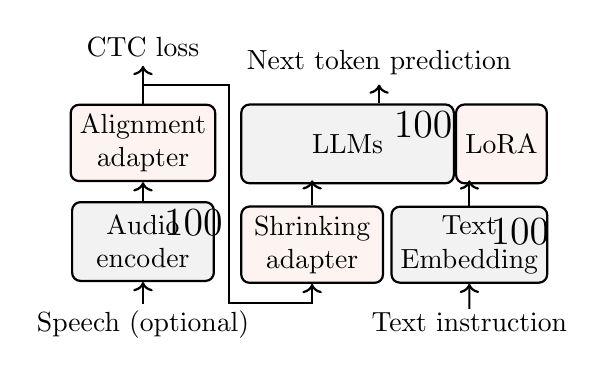
\begin{tikzpicture} [scale=0.8]
        \node(ae) at (0,0) [rectangle, draw=black, fill=gray!10, rounded corners=3pt, thick, minimum width=1.8cm,minimum height=1cm,align=center] {Audio\\encoder};
        \node(freeze) at ([xshift=0.8cm,yshift=0.3cm]ae.center) [rectangle, align=center] {\Large{\ding{100}}};
        \node(fb) at ([yshift=-0.3cm]ae.south) [rectangle, align=center,anchor=north] {Speech (optional)};
        \node(aa) at ([yshift=0.3cm]ae.north) [rectangle, draw=black, fill=orange!10, rounded corners=3pt, thick, minimum width=1.8cm,minimum height=0.5cm,align=center,anchor=south] {Alignment\\adapter};
        \node(ctc) at ([yshift=0.6cm]aa.north) [rectangle,align=center,anchor=south] {CTC loss};
        \node(sa) at ([xshift=0.4cm,yshift=-0.05cm]ae.east) [rectangle, draw=black, fill=orange!10, rounded corners=3pt, thick, minimum width=1.8cm,minimum height=0.5cm,align=center,anchor=west] {Shrinking\\adapter};
        \node(llm) at ([yshift=1.6cm]sa.west) [rectangle, draw=black, fill=gray!10, rounded corners=3pt, thick, minimum width=2.7cm,minimum height=1.0cm,align=center,anchor=west] {LLMs};
        \node(lora) at (llm.east) [rectangle, draw=black, fill=orange!10, rounded corners=3pt, thick, minimum width=1.0cm,minimum height=1.0cm,align=center,anchor=west] {LoRA};
        \node(te) at ([xshift=0.1cm]sa.east) [rectangle, draw=black, fill=gray!10, rounded corners=3pt, thick, minimum width=1.8cm,minimum height=0.5cm,align=center,anchor=west] {Text\\Embedding};
        \node(freeze3) at ([xshift=0.8cm,yshift=0.2cm]te.center) [rectangle, align=center] {\Large{\ding{100}}};
        \node(ti) at ([yshift=-0.3cm]te.south) [rectangle, align=center,anchor=north] {Text instruction};
        \node(freeze2) at ([xshift=1.2cm,yshift=0.3cm]llm.center) [rectangle, align=center] {\Large{\ding{100}}};
        \node(loss) at ([xshift=0.5cm, yshift=0.3cm]llm.north) [rectangle, align=center,anchor=south] {Next token prediction};

        
        \draw[->,thick]([yshift=-0.05cm]fb.north)--(ae.south);
        \draw[->,thick](ae.north)--(aa.south);
        \draw[->,thick](aa.north)--(ctc.south);
        \draw[->,thick](sa.north)--([yshift=0.4cm]sa.north);
        \draw[->,thick](te.north)--([yshift=0.4cm]te.north);
        \draw[->,thick]([yshift=-0.3cm]loss.south)--(loss.south);
        \draw[->,thick]([yshift=-0.1cm]ti.north)--(te.south);

        \draw[->,thick](aa.north)--([yshift=0.3cm]aa.north)--([xshift=0.2cm, yshift=0.3cm]aa.north -| aa.east)--([xshift=0.2cm, yshift=-0.3cm]sa.south -| aa.east)--([yshift=-0.3cm]sa.south)--(sa.south);
      \end{tikzpicture}
    \end{minipage}
    }
    \subfigure[SFT stage]{
    \begin{minipage}[t]{0.20\linewidth}
    \centering
    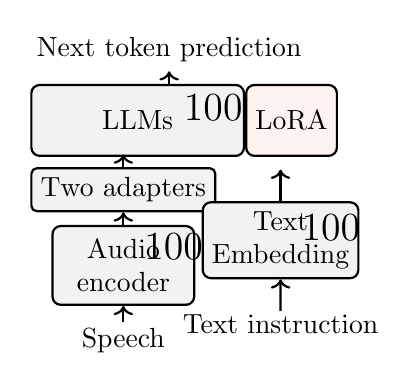
\begin{tikzpicture} [scale=0.8]
        \node(ae) at (0,0) [rectangle, draw=black, fill=gray!10, rounded corners=3pt, thick, minimum width=1.8cm,minimum height=1cm,align=center] {Audio\\encoder};
        \node(freeze) at ([xshift=0.8cm,yshift=0.3cm]ae.center) [rectangle, align=center] {\Large{\ding{100}}};
        \node(fb) at ([yshift=-0.2cm]ae.south) [rectangle, align=center,anchor=north] {Speech};
        \node(aa) at ([yshift=0.2cm]ae.north) [rectangle, draw=black, fill=gray!10, rounded corners=2pt, thick, minimum width=1.8cm,minimum height=0.5cm,align=center,anchor=south] {Two adapters};
        
        \node(llm) at ([yshift=1.1cm]aa.west) [rectangle, draw=black, fill=gray!10, rounded corners=3pt, thick, minimum width=2.7cm,minimum height=0.9cm,align=center,anchor=west] {LLMs};
        \node(lora) at (llm.east) [rectangle, draw=black, fill=orange!10, rounded corners=3pt, thick, minimum width=0.9cm,minimum height=0.9cm,align=center,anchor=west] {LoRA};
        \node(te) at ([xshift=0.1cm,yshift=0.4cm]ae.east) [rectangle, draw=black, fill=gray!10, rounded corners=3pt, thick, minimum width=1.8cm,minimum height=0.5cm,align=center,anchor=west] {Text\\Embedding};
        \node(freeze3) at ([xshift=0.8cm,yshift=0.2cm]te.center) [rectangle, align=center] {\Large{\ding{100}}};
        \node(ti) at ([yshift=-0.4cm]te.south) [rectangle, align=center,anchor=north] {Text instruction};
        \node(freeze2) at ([xshift=1.2cm,yshift=0.2cm]llm.center) [rectangle, align=center] {\Large{\ding{100}}};
        \node(loss) at ([xshift=0.5cm, yshift=0.2cm]llm.north) [rectangle, align=center,anchor=south] {Next token prediction};
       
        \draw[->,thick]([yshift=-0.05cm]fb.north)--(ae.south);
        \draw[->,thick](ae.north)--(aa.south);
        \draw[->,thick](aa.north)--([yshift=0.2cm]aa.north);
        \draw[->,thick](te.north)--([yshift=0.5cm]te.north);
        \draw[->,thick]([yshift=-0.2cm]loss.south)--(loss.south);
        \draw[->,thick]([yshift=-0.1cm]ti.north)--(te.south);
        
      \end{tikzpicture}
    \end{minipage}
    }
      \caption{Training progress of Soundwave. The gray modules are frozen while the orange modules are updated.}
      \label{architecture}
  \end{figure*}

  




\section{Results}
\label{sec:results}
\subsection{Experimental Setup}

\begin{figure*}[ht]
\centering
\begin{minipage}{.49\textwidth}
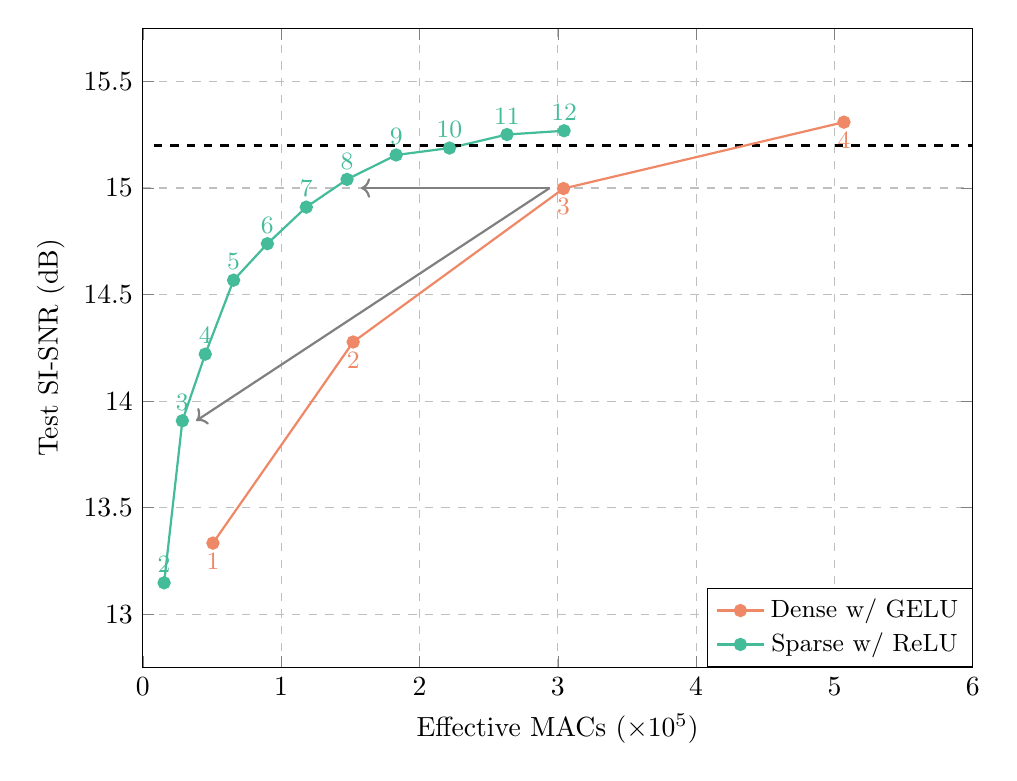
\begin{tikzpicture}
\begin{axis}[
  width=\textwidth,
  height=0.8\textwidth,
  %xmode=log,
  grid=both,
  minor grid style={dashed},
tick label style={/pgf/number format/fixed},
  major grid style={dashed},
  xlabel={Effective MACs ($\times 10^5$)},
  ylabel={Test SI-SNR (\unit{\decibel})},
  legend style={
    at={(1.0,0.0)},   % x,y coordinates relative to the axis
    anchor=south east,
    legend columns=1
  },
  ymax=15.75,
  ymin=12.75,
  tick label style={font=\normalsize},
  label style={font=\normalsize},
  every axis legend/.append style={font=\small},
  xmin=-200,
xtick={0,100000,200000,300000,400000,500000,600000},
xticklabels={{$0$},{$1$},{$2$},{$3$},{$4$},{$5$},{$6$}},
  scaled x ticks=false, 
  xmax=600000
]

    % 2) ReLU, Sparse (blue, dashed, round marker)
    \addplot+[
      forget plot,
      color=mint,
      solid,
      thick,
      mark=*,
      mark options={fill=mint, draw=mint},
      nodes near coords,
      point meta=explicit symbolic,
      every node near coord/.append style={anchor=south, font=\small}
    ] table [meta=label, col sep=space] {
      x      y      label
 15385.396493  13.147347          2
 28589.361895  13.907744          3
 45140.258309 14.220416          4
 65621.998638  14.567575          5
 90050.190476  14.738816          6
118193.413502  14.910501          7
147635.113026  15.040557          8
183166.524831 15.155087          9
221680.248892 15.187635         10
263277.181804  15.251074         11
304559.862373 15.268791         12
    };


    \addplot [
      black,
      dashed,
      thick,
      forget plot
    ] coordinates {(8000,15.2) (9000000,15.2)} 
      node [pos=1, anchor=north east, font=\small] {Previous SotA};


    % 3) GeLU, Dense (red, solid, round marker)
    \addplot+[
      forget plot,
      color=orange,
      solid,
      thick,
      mark=*,
      mark options={fill=orange, draw=orange},
      nodes near coords,
      point meta=explicit symbolic,
      every node near coord/.append style={anchor=north, font=\small}
    ] table [meta=label, col sep=space] {
      x      y      label
  50688.0  13.333696          1
 152064.0  14.277531          2
 304128.0 14.997617          3
 506880.0 15.309213          4
    };

    
    % Weights: Dense (solid black line)
    \addlegendimage{orange, mark=*, solid, thick}
    \addlegendentry{Dense w/ GELU}

    % Weights: Sparse (dashed black line)
    \addlegendimage{mint, mark=*, solid, thick}
    \addlegendentry{Sparse w/ ReLU}

  % Now draw the big red arrows (example):
  %  -- Arrow from orange #1 (x=50688, y=13.3337) to orange #3 (x=304128, y=14.9976)
  \draw[->, thick, black!50]
    (axis cs:294128, 15.0)
    -- (axis cs:157635.113026,  15.0) ;

  %  -- Arrow from orange #3 (x=304128, y=14.9976) to green #9 (x=183166.5248, y=15.1551)
  %     (This arrow angles 'back' to the left, as in your figure.)
  \draw[->,thick, black!50]
    (axis cs:294128, 15.0)
    -- (axis cs:38589.361895,  13.907744);
  \end{axis}
\end{tikzpicture}
\end{minipage}
\begin{minipage}{.49\textwidth}
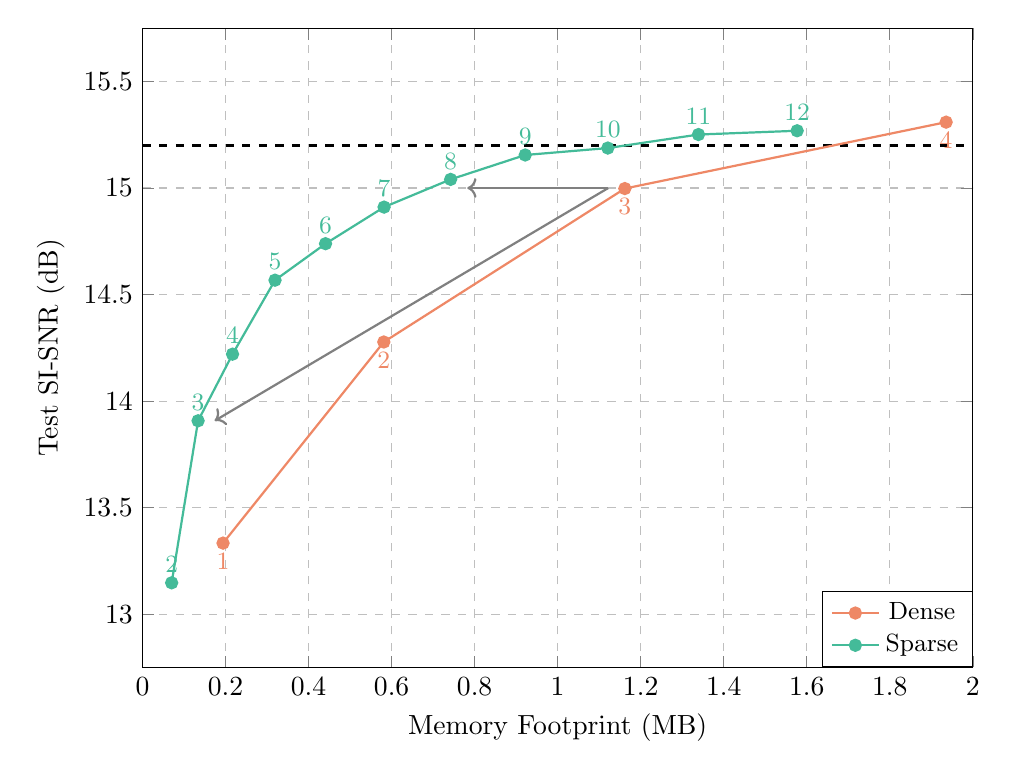
\begin{tikzpicture}
\begin{axis}[
  width=\textwidth,
  height=0.8\textwidth,
  %xmode=log,
  grid=both,
  minor grid style={dashed},
  major grid style={dashed},
  xlabel={Memory Footprint (\unit{\mega\byte})},
  ylabel={Test SI-SNR (\unit{\decibel})},
  legend style={
    at={(1,0)},   % x,y coordinates relative to the axis
    anchor=south east,
    legend columns=1
  },
  ymax=15.75,
  ymin=12.75,
  xmin=0,xmax=2,
  tick label style={font=\normalsize},
  label style={font=\normalsize},
  every axis legend/.append style={font=\small},
]

    \addplot [
      black,
      dashed,
      thick,
      forget plot
    ] coordinates {(0,15.2) (2,15.2)} 
      node [pos=1, anchor=north east, font=\small] {};

    % 4) GeLU, Sparse (red, dashed, round marker)
    \addplot+[
      forget plot,
      color=orange,
      solid,
      thick,
      mark=*,
      mark options={fill=orange, draw=orange},
      nodes near coords,
      point meta=explicit symbolic,
      every node near coord/.append style={anchor=north, font=\small}
    ] table [meta=label, col sep=space] {
      x      y      label
0.193909 13.333696          1
0.581177 14.277531          2
1.161804 14.997617          3
1.935791 15.309213          4
    };

    % 4) GeLU, Sparse (red, dashed, round marker)
    \addplot+[
      forget plot,
      color=mint,
      solid,
      thick,
      mark=*,
      mark options={fill=mint, draw=mint},
      nodes near coords,
      point meta=explicit symbolic,
      every node near coord/.append style={anchor=south, font=\small}
    ] table [meta=label, col sep=space] {
      x      y      label
0.070136 13.147347 2
0.133800 13.907744 3
0.216820 14.220416 4
0.319128 14.567575 5
0.440823 14.738816 6
0.581836 14.910501 7
0.742147 15.040557 8
0.921845 15.155087 9
1.120834 15.187635 10
1.339239 15.251074 11
1.576909 15.268791 12
    };

    % -----------------------------------------------------------
    % Manual legend entries

    % Weights: Dense (solid black line)
    \addlegendimage{orange, mark=*, solid, thick}
    \addlegendentry{Dense}

    % Weights: Sparse (dashed black line)
    \addlegendimage{mint, mark=*, solid, thick}
    \addlegendentry{Sparse}

  \draw[->, thick, black!50]
    (axis cs:1.121804, 15.0)
    -- (axis cs:0.782147,  15.0) ;

  %  -- Arrow from orange #3 (x=304128, y=14.9976) to green #9 (x=183166.5248, y=15.1551)
  %     (This arrow angles 'back' to the left, as in your figure.)
  \draw[->,thick, black!50]
    (axis cs:1.121804, 15.0)
    -- (axis cs:0.173800,  13.907744);
  \end{axis}
\end{tikzpicture}
\end{minipage}
\caption{Pareto fronts for S5 network audio denoising quality (SI-SNR) as a function of effective compute (left) and memory footprint (right) on the Intel N-DNS test set. S5 networks with  weight and activation sparsity (green) exhibit a large domain of Pareto optimality versus dense S5 networks (orange). Number annotations enumerate increasing S5 dimensionality configurations, from \qty{500}{k} to \qty{4}{\million} parameters. Dashed horizontal like marks SI-SNR of Spiking-FullSubNet XL, the previous state-of-the-art model. The horizontal arrows highlight models used for hardware deployment, the diagonal arrows highlight models of the same width. See text for details.}
\label{fig:ndns_performance_efficiency}
\end{figure*}

\paragraph{Software}
We implemented our methodology in JAX 0.4.30, building on top of the original S5 codebase \cite{DBLP:conf/iclr/SmithWL23}, with JaxPruner \cite{DBLP:journals/corr/abs-2304-14082} for the pruning algorithms and the AQT library \cite{aqt} for quantization-aware training. We implemented static quantization and a fixed-point model ourselves using only JAX.
% The implementation on the Intel Loihi 2 is based on NxKernel 0.2.0 and all characterization results are produced on a single-chip Oheo Gulch N3C1 board (accessible only to Intel Neuromorphic Research Community members).
% The implementation on the NVIDIA Jetson Orin Nano 8GB is running Jetpack 6.2, CUDA 12.4, JAX 0.4.32 and using the MAXN SUPER power mode. Power on the Jetson is reported as only CPU\_GPU\_CV through jtop 4.3.0.
% Performance results are based on testing as of Jan 2025 and may not reflect all publicly available security updates. Results may vary.

\paragraph{Audio denoising task}

We evaluated our approach on the Intel Neuromorphic Deep Noise Suppression Challenge \cite{Timcheck_2023}.
%
% AP: We should give a general understanding of the task, the pre-/post-processing steps, the acceptable latency, and the SI-SNR metric.
The objective of the Intel N-DNS Challenge is to enhance the clarity of human speech recorded on a single microphone in a noisy environment.
%
The Intel N-DNS Challenge utilizes data from the Microsoft DNS Challenge,  encompassing clean human speech audio samples and noise source samples.  \cite{reddy2020interspeech, reddy2021icassp, reddy2021interspeech, dubey2024icassp}.
Clean human speech and noise samples are mixed to produce noisy human speech with a ground truth clean human speech goal.

To train our models, we used the default Intel N-DNS Challenge training and validation sets, each consisting of \qty{60000}{} noisy audio samples of \qty{30}{\s} each, and a test set with \qty{12000}{} samples. 
%
We encoded and decoded each audio sample using the Short-Time Fourier Transform (STFT) and Inverse Short-Time Fourier Transformer (iSTFT) \cite{grochenig2013foundations}. 
%
Following the N-DNS baseline solution, NsSDNet \cite{shrestha2024efficient}, we adopted a \qty{32}{\milli\s} window length and a \qty{8}{\milli\s} hop length for the STFT/ISTFT.
%
This resulted in a nominal real-time audio processing latency of \qty{32}{\milli\s}, which allows ample time (\qty{8}{\milli\s}) for denosing network inference, as \qty{40}{\milli\s} is the standard for an acceptable latency as recognized in the Microsoft N-DNS Challenge. 

We evaluated the denoising quality of our model using the scale-invariant signal-to-noise ratio (SI-SNR)
\begin{equation}
    \text{SI-SNR} = 10\log_{10}\frac{\norm{s_\text{target}}^2}{\norm{e_\text{noise}}^2}.
\end{equation}
Importantly, SI-SNR provides a volume-agnostic measure of audio cleanliness relative to the ground truth signal. 



\subsection{Pareto Front of Performance and Efficiency}
\label{ss:pareto-front}

We studied the performance-efficiency Pareto front of dense and sparse models across inference compute budgets.
Starting from the S5 architecture \cite{DBLP:conf/iclr/SmithWL23}, we trained a family of dense models of increasing size by linearly scaling the model dimensions (i.e.\ model width and size of the SSM hidden state), while keeping the depth fixed to three S5 layers.
Similarly, we trained a family of sparse models, i.e., pruned and ReLU-fied, according to our methodology discussed above, with $90\%$ of weights pruned by the end of training (further details on the model dimensions are provided in \Cref{app:model-params}).
The results, reported in \autoref{fig:ndns_performance_efficiency}, compare de-noising performance (SI-SNR) and computational efficiency as measured by effective MACs and memory footprint (see \Cref{supp:macs}).
%
%Furthermore, we applied a hyperparameter search {\color{red} TODO: details of the hyperparameter search methodology?} to ensure a fair representation of the best performance at each network size and in either sparse or dense configuration.
%
%We computed a proxy measure of efficiency for each model by calculating the effective Multiply-And-Accumulate operations (MACs) per time step and the memory footprint (model size).

The results show that sparsification significantly degrades performance when applied to under-parametrized dense models (e.g., sparsifying dense-\qty{3}{} reduces SI-SNR by $7.3\%$).
However, task performance is recovered with increased model dimensions and the accuracy of dense models is matched by larger sparse ones, with fewer MACs and lower memory requirements.
This gives empirical support to theoretical work on the capacity of sparse-and-wide neural networks \cite{golubeva_are_2020}.
For example, sparse-\qty{8}{} model requires \textbf{$\mathbf{2}\boldsymbol{\times}$ lower compute} and \textbf{$\mathbf{36}\boldsymbol{\%}$ lower memory} than the dense-\qty{3}{} model, \textbf{while achieving the same level of accuracy}.
Overall, sparse models constitute the Pareto front of task performance and computational efficiency across compute budgets.

In terms of absolute task performance, we find that the S5 architecture provides state-of-the-art results on audio denoising out of the box.
When compared to Spiking-FullSubNet-XL \cite{10605482}, the Track 1 winner of the Intel N-DNS Challenge with \qty{15.2}{\dB} SI-SNR, our sparse-\qty{11}{} S5 model requires \textbf{$\mathbf{3.2}\boldsymbol{\times}$ lower compute} and \textbf{$\mathbf{5.37}\boldsymbol{\times}$ lower memory} \textbf{iso-accuracy}.
This finding is in line with previous research on audio modeling with state space models \cite{DBLP:conf/icml/GoelGDR22}, and provides additional evidence on the suitability of these architectures for signal processing.
%
%The XL version of the Spiking-FullSubNet network achieves \qty{15.2}{\dB} SI-SNR on the Intel N-DNS Challenge test set, as noted by the horizontal dashed line in \autoref{fig:ndns_performance_efficiency}. 
%
%Our S5 models can achieve \qty{15.2}{\dB} SI-SNR with modest computational cost and memory footprints.
%In comparison, Spiking-FullSubNet XL uses $8.4 \times 10^5$ effective MACs per \qty{8}{\milli\s} timestep and has a memory footprint of \qty{7.02}{\mega\byte}; these computational cost and memory points are much larger than those of our S5 networks shown in \autoref{fig:ndns_performance_efficiency}---beyond the domain displayed in our plots---suggesting strong competitiveness from our S5 networks, especially under consideration of resource constraints.
% 
%We note that the Spiking-FullSubNet network was trained using a loss function that includes other terms in addition to SI-SNR, catering to other audio quality metrics.
%Therefore, Spiking-FullSubNet's results in the Intel N-DNS Challenge does not represent the maximum achievable SI-SNR for the Spiking-FullSubNet architecture.
%
%Nevertheless, Spiking-FullSubNet's results provide an excellent point of comparison, as SI-SNR was one of the main metrics for which Spiking-FullSubNet was optimized.



\paragraph{Interaction of weight and activation sparsity}

An interesting question is what is the interaction between the two types of sparsity, in weights and activations.
\autoref{fig:activation_sparsity} reports the pre-activation sparsity for different layers across the model depth for two ReLU-fied models of the same size (model variant \qty{6}{}), with and without synaptic sparsity.
%
We observe that the synaptic-sparse model exhibits lower activation sparsity across the board, a finding that is consistent across model sizes.
%
In addition, activation sparsity significantly decreases with model depth, both for dense and sparse models.
These phenomena, previously observed in other models \cite{mukherji2024weight}, suggest that, during training, the model compensates the reduced information flow caused by pruning with increased levels of activation.
Additional research on more advanced activation functions would allow for the optimal allocation of MACs, especially those that provide explicit control over sparsity without cross-channel synchronization (e.g.,\ approximate top-k \cite{DBLP:journals/corr/abs-2412-04358}).
% Nonetheless, weight and activation sparsity combine constructively to result in overall effective MAC reductions greater than that of activation sparsity or weight sparsity alone.

%{\color{red} TODO: would need an ablation study or additional Pareto curves to support this statement. Not necessarily necessary to include the curves in the paper, but that we know it is true would be helpful and could be written in in some way.}

%{\color{red} TODO: may wish to move interpretation to discussion} 

\begin{figure}[t]
\centering
    \pgfplotstableread[row sep=\\,col sep=&]{
        idx     & S5Hid & S5Out & GLU   \\
        1       & 80.754554271698  & 49.60111975669861  & 71.89104557037354   \\
        2       & 58.92143249511719  & 29.815730452537537  & 82.44596123695374  \\
        3       & 51.13644599914551  & 34.60754454135895  & 62.65120506286621  \\
    }\mydata

    \pgfplotstableread[row sep=\\,col sep=&]{
        idx     & S5Hid & S5Out & GLU   \\
        1       & 81.3236653804779  & 39.38424289226532   & 60.10604500770569   \\
        2       & 54.60154414176941  & 19.661784172058105  & 70.28757929801941  \\
        3       & 45.402026176452637  & 22.966817021369934  & 47.028326988220215  \\
    }\mydatasparse

    \begin{tikzpicture}
        \begin{axis}[
                ybar,
                bar width=.28cm,
                width=\linewidth,
                height=0.8\linewidth,
                legend style={
                    at={(0,1)},
                    anchor=north west,
                    legend columns=3,
                },
                xtick=data,
                xticklabels={Layer 1, Layer 2, Layer 3},
                xmin=0.5, xmax=3.5,
                ymax=100,
                ylabel={Pre-activation Sparsity (\%)},
                xlabel={Model Depth},
                ytick pos=left,
                grid=both,
                xmajorgrids=false,
                minor grid style={dashed},
                major grid style={dashed},
              tick label style={font=\normalsize},
              label style={font=\normalsize},
              every axis legend/.append style={font=\small},
            ]
            % Define colors for consistency between data and sparse data.
            % First three plots (non-sparse data) without patterns

            \addlegendimage{area legend, fill=mint}
            \addlegendentry{Norm}
            \addlegendimage{area legend, fill=pear}
            \addlegendentry{S5 Out}
            \addlegendimage{area legend, fill=orange}
            \addlegendentry{GLU}
            \addlegendimage{area legend, fill=black}
            \addlegendentry{Dense}
            \addlegendimage{area legend, fill=black, postaction={pattern=crosshatch, pattern color=white}}
            \addlegendentry{Sparse}
            
            \addplot+[fill=mint, draw=mint] table[x=idx,y=S5Hid] {\mydata};
            \addplot+[fill=pear, draw=pear] table[x=idx,y=S5Out] {\mydata};
            \addplot+[fill=orange, draw=orange] table[x=idx,y=GLU] {\mydata};
            
            % Now add the sparse data with the same colors, but with patterns.
            \addplot+[fill=mint, draw=mint, postaction={pattern=crosshatch, pattern color=white}] table[x=idx,y=S5Hid] {\mydatasparse};
            \addplot+[fill=pear, draw=pear, postaction={pattern=crosshatch, pattern color=white}] table[x=idx,y=S5Out] {\mydatasparse};
            \addplot+[fill=orange, draw=orange, postaction={pattern=crosshatch, pattern color=white}] table[x=idx,y=GLU] {\mydatasparse};

        \end{axis}
    \end{tikzpicture}
    \caption{Activation sparsity of ReLU blocks across model depth for a dense-weight model and a sparse-weight model. The sparse-weight model exhibits significantly lower activation sparsity across layers.}
    \label{fig:activation_sparsity}
\end{figure}


\subsection{Hardware Implementation} 
\label{ss:hardware-implementation}

%In order to validate the sparsity gains on real-time inference performance, we implemented our S5 variants on the Intel Loihi 2 neuromorphic chip.


% bar on x-axis shows accuracy
% stars on x-axis (top) is memory footprint (instead of # params)
% 1) baseline - sparse & relu  ---- with or without QAT @ W8A16
% 3) static quantization conversion
% 4) fxp model in jax
% 5) nxkernel on loihi

% two bars of different shape, one with QAT, the other without
% THIS IS FOR ONE MODEL SIZE ONLY!!

\begin{figure}
    \centering
        
    \pgfplotstableread[row sep=\\,col sep=&]{
        idx     & Baseline & WithQAT  \\
        1       & 10.486  &  12.99034   \\
        2       &  11.84137 & 14.201379776000977    \\
        3       & 9.4657  & 14.5627       \\
        4       & 14.84  & 14.70684814453125   \\
    }\mydata

    \begin{tikzpicture}
        \begin{axis}[
                xbar,
                bar width=.45cm,
                  width=0.925\linewidth,
                  height=0.9\linewidth,
                legend style={at={(0,1)},
                    anchor=north west,legend columns=1,},
                ytick=data,
                yticklabels={FPX (Loihi), FXP (Sim), Static Quant, FP32},
                %xmin=0.5, xmax=3.5,
                ymax=5.3,
                ymin=0.45,
                xmax=20,
                xlabel={Test SI-SNR (\unit{\decibel})},
                xtick={10, 12, 14},
                xtick pos=bottom, % Ensure x-ticks appear only at the bottom
                ytick pos=left, % Ensure x-ticks appear only at the bottom
                grid=both,
                ymajorgrids=false,
                minor grid style={dashed},
                major grid style={dashed},
              tick label style={font=\normalsize},
              label style={font=\normalsize},
              every axis legend/.append style={font=\small},
            ]
                \addplot+[
                    sharp plot,
                    stack plots=false,
                    forget plot,
                    color = black,
                    mark = *,
                    thick,
                    fill = none,
                    draw=black,
                  nodes near coords,
                  point meta=explicit symbolic,
                  every node near coord/.append style={anchor=north west, font=\small}
                ]   table [meta=footprint, col sep=space] {
          x      y      footprint
          15.684306   1     \qty{116.7}{}
          15.684306   2     \qty{116.7}{}
          17.644938   3   \qty{451.4}{}
          17.644938   4   \qty{451.4}{}
        };
            \addlegendimage{area legend, fill=mint}
            \addlegendentry{Base}
            \addlegendimage{area legend, fill=mint, postaction={pattern=crosshatch, pattern color=white}}
            \addlegendentry{QAT}
            \addplot+[fill=mint, draw=mint, postaction={pattern=crosshatch, pattern color=white}] table[x=WithQAT,y=idx] {\mydata};
            \addplot+[fill=mint, draw=mint] table[x=Baseline,y=idx] {\mydata};

    \node[fill=white, inner sep=2pt, draw=none] at (17.45,4.75) {Memory (\unit{\kilo\byte})};
        \end{axis}
    \end{tikzpicture}
    \caption{Impact of quantization interventions on Test SI-SNR and memory footprint, with and without quantization-aware training, for model variant sparse-\qty{6}{}.}
    \label{fig:quantization_interventions}
\end{figure}

\paragraph{Impact of fixed-point conversion}

Since Loihi 2 only supports fixed-point (FXP) arithmetic, as presented in \Cref{sec:methodology}, we quantized the weights and activations of our model and implemented the network dynamics in FXP arithmetic. The effect of our quantization methodology is presented in \autoref{fig:quantization_interventions}.
%
Starting from a 32-bit floating-point (FP32) model, we apply static quantization, which rounds weights and activations using fixed scales, but still performs the actual computation in FP32. Notably, Quantization-Aware Training (QAT) is very effective in maintaining test performance (SI-SNR) from FP32 to static quantization, compared to Post-Training Quantization (PTQ).
%
The frozen scales from static quantization are imported into our FXP model implemented in JAX, which uses only int32 types and fixed-point arithmetic to compute the forward pass of the model.
We observe further performance degradation in the FXP simulation, which we analyze in more detail in \Cref{appendix:fxp-sim-mismatch}. 
%
We finally map the FXP model to Loihi 2 and perform inference on the chip, again finding a degradation in SI-SNR, which is likely due to subtle differences in the integer arithmetic performed by the FXP simulation and Loihi 2 implementation with fused layers. Another source of mismatch is that the FXP model in simulation handles overflows by clipping to the maximum value, whereas Loihi 2 ``wraps around'' the value, resulting in a sign inversion.
%
The size of the model decreases by about a factor of 4 when transitioning from FP32 weights to INT8 weights, as shown on the right side of \autoref{fig:quantization_interventions}.



\paragraph{Power and Performance}

\begin{table*}
    \centering
    \caption{Power and performance results$^*$. The Loihi 2 is running a sparse and quantized S5 model, while the Jetson Orin Nano is running a smaller dense S5 model that reaches similar test performance. All measurements are averaged over \qty{8}{} random samples from the test set, each containing \qty{3750}{} time steps. \textcolor{gray}{Gray highlights} denote violation of real-time constraints for the audio denoising task. Best real-time results are \underline{underlined}.}
    \begin{tabular}{l c r r r}
        \toprule
        & \textbf{Mode}  
        & \multicolumn{1}{c}{\textbf{Latency} ($\downarrow$)} 
        & \multicolumn{1}{c}{\textbf{Energy} ($\downarrow$)}
        & \multicolumn{1}{c}{\textbf{Throughput} ($\uparrow$)} \\
        \midrule
        \textbf{Token-by-token}  \\
        \quad Intel Loihi 2$^\dagger$ & Fall-Through              &       \underline{\qty{76}{\micro\second}} &    \underline{\qty{13}{\micro\joule/\token}} &    \underline{\qty{13178}{\token/\second}} \\
        \quad Jetson Orin Nano$^\ddagger$ & Recurrent 1-step $(b=1)$ &     \qty{2688}{\micro\second} &  \qty{15724}{\micro\joule/\token} &  \qty{372}{\token/\second} \\
        \quad Jetson Orin Nano$^\ddagger$ & Recurrent 10-step $(b=1)$ &    \qty{3224}{\micro\second} &  \qty{1936}{\micro\joule/\token} &   \qty{3103}{\token/\second} \\
        \quad Jetson Orin Nano$^\ddagger$ & Recurrent 100-step $(b=1)$ &   \textcolor{gray}{\qty{10653}{\micro\second}} & \qty{626}{\micro\joule/\token} &   \qty{9516}{\token/\second} \\
        \quad Jetson Orin Nano$^\ddagger$ & Recurrent scan $(b=1)$ &       \textcolor{gray}{\qty{236717}{\micro\second}}& \qty{404}{\micro\joule/\token} &   \qty{15845}{\token/\second} \\
        \midrule
        \textbf{Sample-by-sample} \\
        \quad Intel Loihi 2$^\dagger$ & Pipeline &                        \underline{\qty{60.58}{\milli\second}} &   \underline{\qty{185.80}{\milli\joule/\sample}} &   \underline{\qty{16.58}{\sample/\second}} \\
        \quad Jetson Orin Nano$^\ddagger$ & Scan $(b=1)$ &                                \qty{233.48}{\milli\second} &           \qty{1512.60}{\milli\joule/\sample}& \qty{4.28}{\sample/\second} \\
        \quad Jetson Orin Nano$^\ddagger$ & Scan \textcolor{gray}{$(b=b_{\text{max}})$} & \textit{\qty{226.53}{\milli\second}} &  \textit{\qty{5.89}{\milli\joule/\sample}} &  \textit{\qty{1130.09}{\sample/\second}} \\
        \bottomrule
    \end{tabular}
\centering
% \vskip 0.01em 
\begin{minipage}{.9\textwidth}{\tiny \baselineskip=8pt \setstretch{0.6}
%
$^\dagger$ Loihi 2 workloads were characterized on an Oheo Gulch system with N3C1-revision Loihi 2 chips running NxCore 2.5.8 and NxKernel 0.2.0 with on-chip IO unthrottled sequencing of inputs. Researchers interested to run S5 on Loihi 2 can gain access to the software and systems by joining \textit{Intel's Neuromorphic Research Community}.
%
$^\ddagger$ Jetson workloads were characterized on an NVIDIA Jetson Orin Nano 8GB running Jetpack 6.2, CUDA 12.4, JAX 0.4.32, using the MAXN SUPER power mode; energy values are computed based on the TOT power as reported by jtop 4.3.0. The batch size $b_{\text{max}}=256$ was chosen to be the largest that fits into memory.
%
$^*$Performance results are based on testing as of January 2025 and may not reflect all publicly available security updates; results may vary.
}
\end{minipage}
    \label{tab:pnp}
\end{table*}


To measure the empirical efficiency benefits afforded by the sparse S5 model on neuromorphic hardware, we profile inference on Loihi 2 using the fixed-point S5 model, in particular, configuration sparse-\qty{8}{} from \autoref{fig:ndns_performance_efficiency}.
%
To compare to conventional hardware, we profile the smallest dense model that achieves equivalent performance on Jetson Orin Nano\footnote{Our W8A16 fixed-point model in JAX does not provide a speedup over the FP32 model on the Jetson Orin Nano, therefore we profile the FP32 model.}, which is configuration dense-\qty{3}{} from \autoref{fig:ndns_performance_efficiency}.
%
There exist a variety of modes in which to execute a model on Loihi and Jetson, each exhibiting different tradeoffs in terms of latency, throughput, and energy.
Therefore, we present different modes for a comprehensive characterization and comparison.
We summarize our profiling results in \autoref{tab:pnp}. More details on the different execution modes on Loihi 2 are presented in \Cref{app:exmode}.

In real-time, token-by-token processing on a single input sequence, Loihi 2 processes a single STFT frame $\mathbf{35\times}$ \textbf{faster} and with $\mathbf{1200\times}$ \textbf{less energy} than the Jetson Orin Nano. % (Token-by-token; Loihi 2 Fall-Through and Jetson Orin Nano Recurrent 1-step (b=1) in \autoref{tab:pnp}). 
When the Jetson Orin Nano processes ``chunks'' of multiple time steps, its utilization increases, and energy per token improves. With the largest chunks that fit the real-time requirement of latency $\leq$\qty{8}{\milli\sec}, Loihi 2 is \textbf{$\mathbf{42}\times$ faster} and uses \textbf{$\mathbf{149} \times$ less energy} per token.

In offline processing, when many STFT frames are buffered to process in succession (or in parallel), the energy efficiency and throughput of the Jetson Orin Nano improves. Loihi 2 performs offline processing with pipelining (see \Cref{app:exmode} for further explanation). When processing single sequences, \textit{i.e.} batch size $b=1$, Loihi 2 has \textbf{$\mathbf{3.7} \times$ higher throughput} with \textbf{$\mathbf{8}\times$ less energy} per sample. 

It is important to note that the Jetson Orin Nano is only fully utilized when processing \qty{256}{} sequences in parallel, and at this level, it shows significantly higher throughput while consuming less energy per sample, compared to Loihi 2. We include these results in the last row of \autoref{tab:pnp}.

\paragraph{Energy at real-time inference rate}
The latency budget for the neural network component of the audio denoising pipeline, running either on Loihi 2 or on the Jetson, is \qty{8}{\milli\s}.
Our Loihi 2 and Jetson implementations are well below 8ms for online inference.
%
Thus, to estimate the energy consumption in real-time settings, where subsequent tokens are actually \qty{8}{\milli\s} apart, we rescale the power as:
\begin{equation*}
    P_\text{total}^\text{real-time} =  P_\text{static} + \frac{t_\text{compute}}{\qty{8}{\milli\s}} P_\text{dynamic},
\end{equation*}
based on the power measurements in token-by-token processing.
In this setting, Loihi 2 achieves \qty{1128}{\micro\joule/\token} while the Jetson achieves \qty{36528}{\micro\joule/\token} for token-by-token processing and \qty{3720}{\micro\joule/\token} when processing chunks of 10 time steps at once. Loihi 2 remains at least $3 \times$ more energy efficient than the Jetson Orin Nano.

\paragraph{Limitations}

Our Jetson Orin Nano implementation is in FP32, while our Loihi 2 implementation is in W8A16. Our fixed-point model in JAX provides no improvements in runtime or energy. More competitive Jetson energy, latency, and throughput could potentially be obtained by developing a more optimized quantized implementation. 

% \paragraph{Energy and throughput for offline processing}

% {\color{red} TODO: Distill this discussion in the PnP comparison and remove this paragraph.

% If we move from online processing to offline processing, i.e., buffer several STFT frames to rapidly process in succession, Jetson energy efficiency and throughput improves (Jetson Orin Nano, Recurrent $n$-step or Recurrent scan).
% %
% However, this comes at the cost of buffering and additional processing latency. 
% %
% Jetson Orin Nano can also perform offline S5 utilizing a parallel scan routine (Sample-by-sample, Jetson Orin Nano, Scan); here, batch processing improves Jetson throughput and energy as well (b = max). 
% %
% Nonetheless, Loihi 2 performs offline processing in pipelined mode for batch size 1 with approximately $3.8\times$ increase in throughput and approximately $24\%$ increased energy cost compared to the most efficient batch size 1 Jetson implementation, which is the recurrent scan.
% %
% When using the maximal batch size than can fit on the Jetson's memory, however, the Jetson parallel scan implementation achieves the highest throughput of approximately 4.2M tokens per second, \textcolor{red}{yet at a substantial energy cost per token}.
% }



\section{Discussion}
\label{sec:discussion}
\section{Discussion}

This study presents PathFinder, a multi-modal, multi-agent AI framework designed to emulate the multi-scale, iterative diagnostic approach of expert pathologists for histopathology whole slide images (WSIs). By integrating Triage, Navigation, Description, and Diagnosis Agents, PathFinder collaboratively gathers evidence to deliver accurate, interpretable diagnoses with natural language explanations. Notably, it surpasses state-of-the-art methods and the average performance of human experts in melanoma diagnosis, setting a new benchmark in AI-driven pathology.

PathFinder has the potential to accelerate diagnostic workflows, reducing the reliance on manual examination and enabling timely patient care in clinical settings. Its natural language descriptions provide interpretability, facilitating the validation of AI-generated diagnoses by pathologists. Moreover, its integration of vision-language models (VLMs) and large language models (LLMs) highlights the promise of multi-modal AI in delivering scalable, specialized diagnostic tools that could improve access to pathology expertise.

\noindent\textbf{Limitations.} Despite its strengths, PathFinder has limitations. The framework relies on pre-existing datasets and significant computational resources, posing challenges in resource-constrained environments. Additionally, the complexity of the Navigation Agent’s decision-making process and occasional hallucinations by the Description Agent could affect transparency and accuracy of the decision-making process. Future work should address these issues by enhancing dataset diversity, computational efficiency, and patch selection strategies, further advancing PathFinder's potential as a transformative tool in AI-assisted pathology.




\section*{Author Contributions}

A.\ P.\ and S.A.\ drove the project conception, developed the initial codebase for training and analyzing sparse S5 models, run the training experiments, and developed the Loihi implementation.
A.\ P.\ implemented the sparsification methods and an early prototype on the chip, and collected benchmarking results on Loihi.
S.\ A.\ implemented the quantization methods and the fixed-point model and benchmarked the dense models on the Jetson board.
J.\ T.\ and P.\ S.\ helped evaluating the Loihi implementation.
J.\ T.\ integrated the audio denoising task in the training codebase.
A.\ W.\ provided general guidance on the scope of the project.
S.\ B.\ S.\ provided technical guidance for the fixed-point and Loihi implementations.
All authors contributed to writing and reviewing the paper.



\bibliography{BIBLIOGRAPHY}
\bibliographystyle{icml2024}

\clearpage
\appendix
\section{Supplemental Material}
\label{sec:appendix}
\section{Data Sourcing Details}
Our dataset is constructed using current data sources to ensure spatio-temporal consistency and personalization. Below, we detail the sourcing methodology and heuristics for each component:

\subsection{Restaurants}  
We extracted restaurant details using \textbf{TripAdvisor’s Apify scraper}\footnote{\url{https://console.apify.com/actors/dbEyMBriog95Fv8CW/input}}, which provided all necessary attributes except precise pricing. TripAdvisor denotes cost using dollar symbols (\$–\$\$\$) instead of exact values. To estimate absolute prices, we leveraged city-specific restaurant price indices from \textbf{Numbeo}\footnote{\url{https://www.numbeo.com/cost-of-living/}}, scaling them according to the number of dollar symbols in each price rating.  

\subsection{Attractions}  
Attraction details, including subcategories, were sourced from \textbf{TripAdvisor’s Apify scraper}\footnote{\url{https://console.apify.com/actors/dbEyMBriog95Fv8CW/input}}. Since a majority of attractions lacked predefined visit durations, we consulted domain experts to establish category-wise average durations for each attraction type. Finally, each attraction’s duration was assigned as the mean of the categories it belonged to, ensuring a realistic time allocation (Table \ref{tab:subcategory_duration}).

\subsection{Flights}  
We adopted the \cite{xie2024travelplanner} flight database but adjusted all dates to November 2024 to maximize temporal alignment with event data. This adjustment ensures that LLM-generated itineraries incorporate relevant event-based recommendations.  

\subsection{Distance Matrices}  
All pairwise distances were computed using \textbf{OpenStreetMap’s OSRM API}\footnote{\url{http://project-osrm.org/}}, ensuring accurate and real-time routing information.  

\subsection{Accommodations}  
We scraped accommodation listings from Airbnb using \textbf{Apify’s Airbnb scraper}\footnote{\url{https://apify.com/dtrungtin/airbnb-scraper}}. Since minimum stay requirements were not available in the extracted data, we excluded this attribute from our dataset.  

\subsection{Events}  
Event data was collected using \textbf{Ticketmaster’s Apify scraper}\footnote{\url{https://console.apify.com/actors/Hi7bNMx0vqaqvdfZQ}}, covering a diverse range of concerts, sports, theater, and other entertainment events.  

\subsection{Public Transit}  
We sourced transit schedules from the \textbf{General Transit Feed Specification (GTFS)}\footnote{\url{https://gtfs.org/}} for 140 cities. For each Point of Interest (PoI)—including accommodations, restaurants, and attractions—we determined the nearest public transit stop using geodesic distance (computed via \textbf{Geopy}). This enables LLMs to incorporate realistic public transit connectivity when generating travel itineraries. 

\begin{table}[h]
    \centering
    \renewcommand{\arraystretch}{0.9}
    \setlength{\tabcolsep}{8pt} % Adjust column spacing
    \begin{tabular}{l c}
        \toprule
        \textbf{Category} & \textbf{Duration (hrs)} \\
        \midrule
        Boat Tours \& Water Sports & 3.5 \\
        Casinos \& Gambling & 2.5 \\
        Classes \& Workshops & 1.5 \\
        Concerts \& Shows & 2.5 \\
        Food \& Drink & 2.5 \\
        Fun \& Games & 1.5 \\
        Museums & 3.0 \\
        Nature \& Parks & 4.5 \\
        Nightlife & 2.5 \\
        Outdoor Activities & 4.0 \\
        Shopping & 1.5 \\
        Sights \& Landmarks & 3.0 \\
        Spas \& Wellness & 2.0 \\
        Water \& Amusement Parks & 5.0 \\
        Zoos \& Aquariums & 2.5 \\
        \bottomrule
    \end{tabular}
    \caption{Attraction visiting duration (hrs) for each category. Note that an attraction can belong to one or more than one categories.}
    \label{tab:subcategory_duration}
\end{table}



\begin{table*}[h]
    \centering
    \renewcommand{\arraystretch}{1.05}
    \begin{tabular}{|p{4cm}|p{11cm}|}
        \hline
        \textbf{Constraint} & \textbf{Description} \\
        \hline
        \multicolumn{2}{|c|}{\cellcolor{gray!25} \textit{Environment Constraint}} \\
        \hline \rule{0pt}{2.5ex}Unavailable Transportation & There is no available flight or driving information between the two cities.  \\
        % \hline
        Unavailable Attractions & There is no available attraction information in the queried city. \\
        \hline
        \multicolumn{2}{|c|}{\cellcolor{gray!25} \textit{Commonsense Constraint}} \\
        \hline \rule{0pt}{2.5ex}Within Sandbox & All information in the plan must be within the closed sandbox; otherwise, it will be considered a hallucination. \\
        Complete Information & No key information should be left out of the plan, such as the lack of accommodation during travel. \\
        Sufficient Meal Gaps (+) & Meal timings must have a minimum
        gap of four hours between breakfast, lunch, and
        dinner to maintain a natural schedule. \\
        Valid PoI list (+) & The
        point-of-interest (PoI) list must follow strict validity rules: each day’s itinerary must begin and end at the designated accommodation, except on the final day when the traveler departs. The list should be limited to accommodations, attractions, and restaurants, ensuring adequate time gaps between flight arrivals and accommodation check-ins, as well as between accommodation check-outs and departures. \\
        Diverse Events (+) & Event choices should not be repeated throughout the trip. \\
        Within Current City & All scheduled activities for the day must be located within that day’s city(ies). \\
        Reasonable City Route & Changes in cities during the trip must be reasonable. \\
        Diverse Restaurants & Restaurant choices should not be repeated throughout the trip. \\
        Diverse Attractions & Attraction choices should not be repeated throughout the trip. \\
        Non-conf. Transportation & Transportation choices within the trip must be reasonable. For example, having both “self-driving” and “flight” would be considered a conflict. \\
        \hline
        \multicolumn{2}{|c|}{\cellcolor{gray!25} \textit{Hard Constraint}} \\
        \hline \rule{0pt}{2.5ex}Budget & The total budget of the trip. \\
        Room Rule & Room rules include “No parties”, “No smoking”, “No children under 10”, “No pets”, and “No visitors”. \\
        Room Type & Room types include “Entire Room”, “Private Room”, “Shared Room”, and “No Shared Room”. \\
        Cuisine & Cuisines include “Chinese”, “American”, “Italian”, “Mexican”, “Indian”, “Mediterranean”, and “French”. \\
        Transportation & Transportation options include “No flight” and “No self-driving”. \\
        Event Types (+) & Event Types include four distinct categories—Sports, Arts \& Theatre, Music, and Film. \\
        Attraction Types (+) &  Each attraction belongs to one or more of 15 predefined categories, ensuring a well-distributed selection of activities. \\
        \hline
        \multicolumn{2}{|c|}{\cellcolor{gray!25} \textit{Persona Components}} \\
        \hline \rule{0pt}{2.5ex}Traveler Type (+) & Defines how a traveler approaches their journey—whether they seek relaxation in cozy spots or adrenaline-pumping adventures. \\
        Purpose of Travel (+) &  Captures the main motivation behind the trip, whether it’s to unwind, seek thrills, explore cultures, or connect with nature. \\
        Spending Preference (+) &  Reflects the traveler’s budget and style, from luxurious indulgence to cost-conscious experiences. \\
        Location Preference (+) &  Highlights preferred environments, such as beaches, mountains, cities, or wildlife-rich forests. \\
        \hline
    \end{tabular}
    \caption{\textit{Comprehensive Constraint and Persona Description. (+) denotes the ones we have added.} }
    \label{tab:full_const_detail}
\end{table*}

\begin{table*}[h]
    \centering
    \renewcommand{\arraystretch}{1}
    \setlength{\tabcolsep}{2pt} % Adjust column spacing
    \begin{tabularx}{\columnwidth}{l *{3}{>{\centering\arraybackslash}X}}
        \toprule
        \textbf{Parameter} & \textbf{3-day} & \textbf{5-day} & \textbf{7-day} \\
        \midrule
        \multicolumn{4}{c}{\textbf{Restaurant Parameters}} \\
        \midrule
        \textbf{Breakfast} & & & \\
        Mean Time & 9.63 & 9.80 & 9.84 \\ 
        Mean Duration (hrs) & 0.90 & 1.08 & 0.85 \\ 
        Std. Time & 1.08 & 1.08 & 1.34 \\ 
        Std. Duration (hrs) & 0.24 & 1.43 & 0.23 \\ 
        Beta & 0.21 & 0.63 & 0.03 \\ 
        \midrule
        \textbf{Lunch} & & & \\
        Mean Time & 14.30 & 14.46 & 14.44 \\ 
        Mean Duration (hrs) & 1.11 & 1.10 & 0.99 \\ 
        Std. Time & 1.03 & 1.07 & 1.07 \\ 
        Std. Duration (hrs) & 0.36 & 0.35 & 0.26 \\ 
        Beta & 0.10 & 0.04 & 0.30 \\ 
        \midrule
        \textbf{Dinner} & & & \\
        Mean Time & 20.75 & 20.67 & 20.42 \\ 
        Mean Duration (hrs) & 1.19 & 1.32 & 1.15 \\ 
        Std. Time & 1.25 & 1.37 & 1.66 \\ 
        Std. Duration (hrs) & 0.43 & 0.91 & 1.15 \\ 
        Beta & -0.20 & -0.18 & -0.07 \\ 
        \midrule
        \multicolumn{4}{c}{\textbf{Attraction Parameters}} \\
        \midrule
        $\lambda_{laidback}$ & 1.10 & 1.26 & 1.11 \\ 
        $\lambda_{adventurous}$ & 2.01 & 1.61 & 1.82 \\ 
        $\sigma_d$ (hrs) & 1.11 & 1.07 & 0.90 \\ 
        $n^{max}$ & 5 & 4 & 4 \\ 
        $n^{min}$ & 0 & 0 & 0 \\ 
        $k$ (hrs) & 0.28 & 0.28 & 0.28 \\ 
        \bottomrule
    \end{tabularx}
    \caption{A comprehensive list of parameter details for 3-day, 5-day, and 7-day scenarios as calculated from the annotation distribution statistics.}
    \label{tab:parameter_details}
\end{table*}





\end{document}